% This nuaa-JUB.tex is a latex-beamer template using the JUB beamer theme produced by Billy Okal.
% URL: https://github.com/makokal/beamer-themes/tree/master/JUB
% 
% Copyright (c) 2011-2014, Billy Okal All rights reserved.
% 
% Redistribution and use in source and binary forms, with or without modification, are permitted provided that the following conditions are met:
% Redistributions of source code must retain the above copyright notice, this list of conditions and the following disclaimer.
% Redistributions in binary form must reproduce the above copyright notice, this list of conditions and the following disclaimer in the documentation and/or other materials provided with the distribution.
% Neither the name of the nor the names of its contributors may be used to endorse or promote products derived from this software without specific prior written permission.
%
% THIS SOFTWARE IS PROVIDED BY THE COPYRIGHT HOLDERS AND CONTRIBUTORS "AS IS" AND ANY EXPRESS OR IMPLIED WARRANTIES, INCLUDING, BUT NOT LIMITED TO, THE IMPLIED WARRANTIES OF MERCHANTABILITY AND FITNESS FOR A PARTICULAR PURPOSE ARE DISCLAIMED. IN NO EVENT SHALL BE LIABLE FOR ANY DIRECT, INDIRECT, INCIDENTAL, SPECIAL, EXEMPLARY, OR CONSEQUENTIAL DAMAGES (INCLUDING, BUT NOT LIMITED TO, PROCUREMENT OF SUBSTITUTE GOODS OR SERVICES; LOSS OF USE, DATA, OR PROFITS; OR BUSINESS INTERRUPTION) HOWEVER CAUSED AND ON ANY THEORY OF LIABILITY, WHETHER IN CONTRACT, STRICT LIABILITY, OR TORT (INCLUDING NEGLIGENCE OR OTHERWISE) ARISING IN ANY WAY OUT OF THE USE OF THIS SOFTWARE, EVEN IF ADVISED OF THE POSSIBILITY OF SUCH DAMAGE.
  
% Required files to compile:
% 1. automation_logo.pdf
% 2. beamerthemeJUB.sty
% 3. bibliography_file.bib
% 4. jjlogo.pdf
% 5. large-corner.pdf
% 6. nuaa.png
% 7. small-corner.pdf
 
% \documentclass[handout]{beamer}
\documentclass{beamer} 

\usetheme{JUB}
%\usepackage{CJKutf8}
\usepackage[UTF8]{ctex}  
\usepackage{booktabs}
%导入 ctex 宏包,添加中文支持
%\usepackage[utf8]{inputenc}
\usepackage[T1]{fontenc}
\usepackage[scaled]{helvet}
\usepackage{libertine}

%简单的插入三种大小的图片的命令
\newcommand{\maxpic}[2]{  \begin{figure}[H]
  \centering
  \includegraphics[width=\textwidth]{./pic/#1}\\
  \caption{#2}
\end{figure}}

\newcommand{\midpic}[2]{  \begin{figure}[H]
  \centering
  \includegraphics[width=0.5\textwidth]{./pic/#1}\\
  \caption{#2}
\end{figure}}

\newcommand{\minpic}[2]{  \begin{figure}[H]
  \centering
  \includegraphics[width=0.2\textwidth]{./pic/#1}\\
  \caption{#2}
\end{figure}}

%插入双栏图片的命令
\newcommand{\doublepic}[4]{ \begin{figure}[H]
\begin{minipage}[H]{0.45\textwidth}
\centering
\includegraphics[width=\textwidth]{./pic/#1}
\caption{#2}
\end{minipage}
\begin{minipage}[H]{0.45\textwidth}
\centering
\includegraphics[width=\textwidth]{./pic/#3}
\caption{#4}
\end{minipage}
\end{figure}}

\begin{document} 
%\begin{CJK*}{UTF8}{gbsn} % support for Chinese

  \title{CT系统参数标定及成像}
  %\subtitle{Subtitle  副标题} % optional
  \author{黄璐哲,方天庆,帅青}
  \date{\today}
  \institute{浙江大学} % optional

  \begin{frame}[plain,t]
    \titlepage
  \end{frame} 
  
  \begin{frame}{Table of Contents 目录}
    \tableofcontents
  \end{frame} 
  
  \section{问题重述}
  \begin{frame}{问题背景}
    CT系统是一种利用样品对射线的能量吸收特性对样品进行断层成像的技术,在不破坏样品的情况下获取样品内部的结构信息。问题中使用的是一种二维CT系统,探测器平面发出平行入射的X射线,探测器绕某固定的旋转中心逆时针旋转180次,可以获得180组接收信息,每组信息有512个等距单元的数据。
  \end{frame} % 

  \begin{frame}{解决的问题}
    我们需要建立数学模型和算法,解决以下问题:
    \begin{enumerate}
    
    \item 标定参数
    
    \item 重构图像
    \item 精度与稳定性分析
    \item 设计新模板
    \end{enumerate}
  \end{frame} % 

  \section{问题一的求解}
  
  \begin{frame}{求解思路}
    \begin{enumerate}
      \item 通过部分数据初步获得模型信息
      \item 建立完整模型
      \item 迭代求解拟合模型
    \end{enumerate}
    \doublepic{fujian1.png}{附件1几何形状}{fujian2.png}{附件2信息}
  \end{frame}

  \begin{frame}{初步计算参数}
    截取圆的部分,得到一组探测信息\(D(i)\),对于探测点\(i\),其发出的射线与圆心的距离为\(d_i = i\Delta d + d_0\),其中\(\Delta d\)为探测器上的射线间距,\(d_0\)为探测器位置相对偏置。那么第\(i\)条射线与圆相交的弦长为\(2\sqrt{R^2 - d_i^2}\),其中R为圆半径。我们推测探测器的接收数据与\(\rho l\)成一次函数关系,即
    \begin{equation}
      D(i)  = \mu\times 2\sqrt{R^2 - ( i\Delta d + d_0)^2}\rho  +c
    \end{equation}
      使用最小二乘法对曲线进行拟合,求出各个参数的值为:
      \[\mu =1.7724 , \Delta d = 0.2768, d_0 = -4.0688, c = 0.0000\]
  \end{frame}
 
  \begin{frame}{初步计算参数}
    \maxpic{fitCir.png}{拟合圆上的数据}
  \end{frame}

  \begin{frame}{完整模型建立}
    以正方形托盘的中心为坐标原点,椭圆中心与圆中心的连线方向为\(x\)轴,过坐标原点垂直于\(x\)轴方向为\(y\)轴,建立平面直角坐标系。在这一坐标系中,设CT系统的旋转中心坐标为\(R(x_0,y_0)\),探测器平面与\(x\)轴的夹角为\(\theta\),探测器中心与旋转中心在探测器平面上的投影的距离为\(d_0\)。
    
  \end{frame}
  
  \begin{frame}{参数定义}
    \begin{figure}
      \begin{center}
        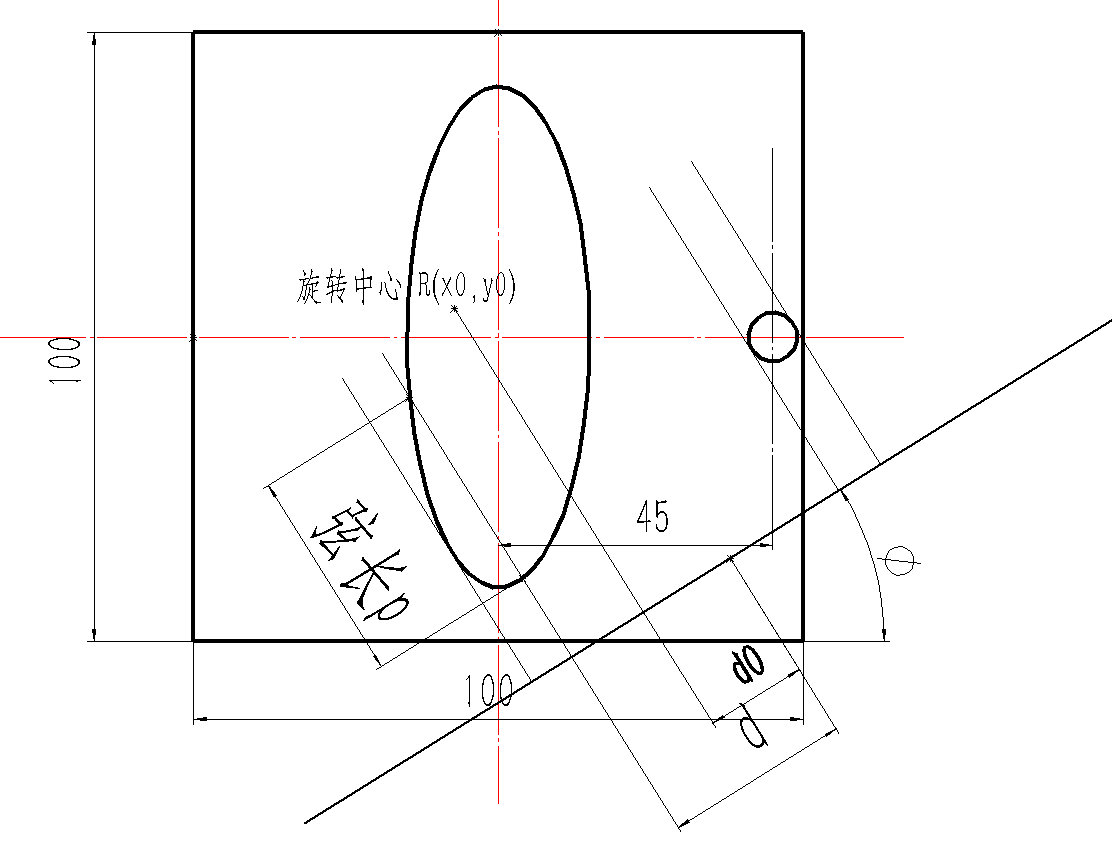
\includegraphics[scale=0.3]{pic/q13.png}
      \end{center}
      \caption{参数定义}
      \label{Fig:xian}
    \end{figure}
  \end{frame}

  \begin{frame}{求解长度}
    标定模板中,椭圆与圆的方程分别为:
    \[\frac{x^2}{m^2} + \frac{y^2}{n^2} = 1,m = 15,n = 40;(x - 45)^2 + y^2 = 4^2\]
    综合求解,所以对于探测角度为\(\phi\)的探测器,其上第\(i\)条X射线探测所得的数值的计算公式为:
    \begin{tiny}
      \begin{align*}\label{va}
      V = & \mu\frac{2mn\sqrt{\max(0,m^2\cos^2\phi + n^2\sin^2\phi - (x_0\cos\phi + y_0\sin\phi + d_0 +  (i - 256.5)\Delta d)^2})}{ m^2\cos^2\phi + n^2\sin^2\phi} \\
        & + 2\mu\sqrt{\max(0,r_0^2 - (G\cos\phi - (x_0\cos\phi + y_0\sin\phi + d_0 +  (i - 256.5)\Delta d))^2)}
      \end{align*}
    \end{tiny}
  \end{frame}

  \begin{frame}{模型求解}
    \begin{itemize}
      \item 选取参数\(d_0,x_0,y_0,\mu,\Delta d,\phi_i,i=1,\ldots,180\)的初值,这里参数的初值可以随意选取,我们设置为\(d_0 = x_0 = y_0 =  0,\mu = 1.7724\)(由前文初步计算得),使用\(512\times 180\)组数据,对所有参数进行拟合,获得第一次求解的参数结果。
      \item 对第一次求解得到的\(\phi_{1_i},i=1,\ldots,180\),对数据进行平滑处理,接着将\(\phi_i\)作为已知参数,使用\(512\times 180\)组数据,以第一次求解的结果作为初值,对参数\(d_0,x_0,y_0,\mu,\Delta d\)进行求解,得到第二次参数的求解结果。
    \end{itemize}
    \end{frame}
    % 局部加权回归散点平滑法是什么
    % 为什么要平滑

    \begin{frame}
    \begin{itemize}
      \item 使用第二次求解得到的参数\(d_0,x_0,y_0,\mu,\Delta d\)作为已知参数,对于180组,每组512个数据,以第(2)步中得到的角度作为初值,分别对每组数据的角度参数进行求解,得到第(3)步的求解结果。
      \item 使用第(2)步与第(3)步的结果作为初始值,再次使用\(512\times 180\)组数据,对所有参数进行拟合,得到最终结果。
      \end{itemize}
      经测试,经过这样几次求解之后,所得值已经稳定,再次求解结果不会有明显改变。
      % 得说明一下继续迭代结果保持稳定
      % 妈的这里好像没法跨页写enumerate
  \end{frame}

  \begin{frame}{求解结果} 
    使用上述算法对模型进行求解,得到各个参数如下:
    \[\mu = 1.7727,x_0 = -9.2696,y_0 = 6.2738\]
    \[d_0 = 0.0000,\Delta d = 0.2768\]
    根据所建坐标系 ,CT系统X射线逆时针旋转的始值为-60.3465$^\circ$,终值 118.6439$^\circ$。
  \end{frame}
  
  \section{问题二的求解}
  \section{问题三的求解}
  \section{问题四的求解}
  %\label{Sec:introduction}
  \begin{frame}{1. Introduction 引言}
    \framesubtitle{frame subtitle 页面副标题}
    This nuaa-JUB.tex is a \LaTeX \ Beamer template using the JUB Beamer theme  produced by Billy Okal.

    \bigskip

    此nuaa-JUB.tex文件是一个使用了Billy Okal制作的JUB Beam主题的\LaTeX \ Beamer模板。

    \begin{figure}
      \begin{center}
        
\includegraphics[scale=0.1]{latex.png}
      \end{center}
      \caption{\LaTeX \ beamer}
      \label{Fig:latex_beamer}
    \end{figure}
  \end{frame} % 

  \section{Mathematical model}
  \label{Sec:model}
  \begin{frame}{2. Mathematical model 数学模型}
    Lists 列表

    \begin{itemize}
    \item Apple
    \item Orange
    \item Banana
    \end{itemize}

    \begin{enumerate}
    \item Monday
    \item Tuesday
    \item Wednesday
    \end{enumerate}

    \begin{description}
    \item[Description list] is a type of list to describe items.
    \item[Description list] 是一种用于描述的列表。
    \end{description}
  \end{frame} 

  \section{Empirical experiments}
  \label{Sec:experiments}
  \begin{frame}{3. Empirical experiments 实验}
    Blocks 区块

      \begin{definition}[Pythagorean theorem]
        The Pythagorean theorem is a fundamental relation in Euclidean geometry among the three sides of a right triangle.
      \end{definition}

      \begin{theorem}[Pythagorean theorem]
        $a^2 + b^2 = c^2$
      \end{theorem}
  \end{frame} 

  \begin{frame}{3. Empirical experiments 实验}
    Blocks 区块

      \begin{exampleblock}{For example}
        $3^2 + 4^2 = 5^2$
      \end{exampleblock}

      \begin{alertblock}{Note}
         Note that the Pythagorean theorem can only be applied to right triangles.
      \end{alertblock}
  \end{frame} 

  \begin{frame}
    \begin{center}
      \Huge{\bf{Thank you!}}
    \end{center}
  \end{frame} % ================================================================
  \section{参考文献}
  \begin{frame}{参考文献}
    \begin{thebibliography}{0}
      
      \bibitem{toumo}
      Kak A C. BOOKS AND PUBLICATIONS:"Principles of Computerized Tomographic Imaging"[J]. Medical Physics, 2002, 29(1):107.
      
      \bibitem{nlm}
      J. Huang et al, "Sparse angular CT reconstruction using non-local means based iterative-correction POCS," Computers in Biology and Medicine, vol. 41, (4), pp. 195-205, 2011.
      
      \bibitem{ct1}庄天戈. CT原理与算法[M]. 上海交通大学出版社, 1992.
      \bibitem{radon}林世明, W.-M.Boerner. 离散Radon变换[J]. 西北工业大学学报, 1988(2):49-56.
      \end{thebibliography}
  \end{frame} % 

  \bibliographystyle{IEEEtran} % comment this line if nothing is cited
  \bibliography{bibliography_file} % comment this line if nothing is cited

%\end{CJK*}
\end{document}